\documentclass[11pt,a4paper]{article}
\usepackage[utf8]{inputenc}
\usepackage[T1]{fontenc}
\usepackage{geometry}
\usepackage{booktabs}
\usepackage{graphicx}
\usepackage{float}
\usepackage{amsmath}
\usepackage{url}
\geometry{margin=2.5cm}
\graphicspath{{../codigo/salidas/}}

\title{Riesgo de Incumplimiento Crediticio\\Regresión Logística en el Contexto Latinoamericano\\[0.4em]
\large Segunda Entrega --- Proyecto Integrador}
\author{Isabella Pensamiento \and Juan Angel Triana}
\date{Machine Learning I --- Profesora Juliana De Mier\\Bogotá D.C., Colombia --- Octubre de 2026}

\begin{document}
\maketitle
\thispagestyle{empty}
\setcounter{page}{1}

\section{Ajustes a la primera entrega}

Antes de modelar, corregimos seis puntos que nos señaló la profesora. Los resumimos aquí y los desarrollamos en las secciones siguientes.

\begin{enumerate}
  \item Definimos de forma explícita qué significa \texttt{mora} (sección~2).
  \item Definimos el momento en que se haría la predicción (sección~2).
  \item Revisamos si \texttt{atraso}, \texttt{clasif\_sbs} y \texttt{score} pueden filtrar la respuesta (sección~3).
  \item Reformulamos la pregunta como una pregunta predictiva (sección~2).
  \item Quitamos la regla de ``Precision superior al 70\%'', porque ese número depende de cuántos morosos hay en la muestra y no de la calidad del modelo. Ahora cada modelo se juzga con el AUC, el PR-AUC y con los tipos de error que comete (sección~6).
  \item Mejoramos la explicación de los supuestos de la regresión logística (sección~8).
\end{enumerate}

Además, algunas decisiones del plan original cambiaron al revisar los datos y lo visto en clase. La Tabla~\ref{tab:cambios} resume qué cambió y por qué. Mantuvimos la línea base del clasificador de mayoría. Todo el código está en el notebook que acompaña este informe, y todas las cifras salen de ahí.

\begin{table}[H]
  \centering
  \caption{Cambios frente al plan de la primera entrega.}
  \label{tab:cambios}
  \small
  \begin{tabular}{@{}p{2.2cm}p{4.2cm}p{6.8cm}@{}}
    \toprule
    Tema & Primera entrega & Ahora y por qué \\
    \midrule
    Modelos & Regresión logística, Ridge/Lasso, LDA y KNN & Logística, LDA, KNN y Naive Bayes. Ridge/Lasso y QDA quedan para la entrega final \\
    Naive Bayes & Fuera de los principales, por suponer independencia & Sigue sin ser principal; entra solo como contraste \\
    Balanceo & Evaluar si conviene & Cinco opciones probadas; el AUC no mejora, se entrena sin balancear \\
    Imputación & Mediana & Mediana más indicador de faltante \\
    Variables & 13 predictores & Escenario principal de 11, sin \texttt{atraso} ni \texttt{clasif\_sbs} \\
    Métricas & AUC y meta de precision & AUC y PR-AUC; sin metas fijas frente a la línea base \\
    Pregunta & Qué características aumentan la probabilidad de mora & Qué tan bien puede predecirse el riesgo de mora \\
    \bottomrule
  \end{tabular}
\end{table}

\section{Pregunta, definición de \texttt{mora} y momento de predicción}

\textbf{Pregunta.} Cambiamos la pregunta de la primera entrega por una predictiva: ¿qué tan bien puede predecirse el riesgo de mora de un cliente de crédito de consumo a partir de información financiera y socioeconómica disponible previamente? Primero medimos qué tan bien se predice; después interpretamos variables, sin tratar los coeficientes como causas.

\textbf{Qué significa \texttt{mora}.} La descripción del autor habla de pagador al día o cliente moroso, pero no trae diccionario de datos. Comprobamos que \texttt{mora} no es lo mismo que tener atraso hoy: el 57,7\% de los clientes con \texttt{mora = 1} tiene \texttt{atraso = 0}, y el 27,2\% de los con \texttt{mora = 0} sí tiene días de atraso. Por eso usamos esta definición operativa:
\begin{quote}
\texttt{mora = 1} significa que el cliente aparece marcado como moroso en la base; \texttt{mora = 0} que aparece como pagador al día.
\end{quote}
Es un supuesto nuestro y lo dejamos como limitación.

\textbf{Momento de predicción.} Pensamos el modelo para cuando el banco evalúa al cliente: conoce perfil, historial y \texttt{score}, pero aún no sabe si quedará marcado como moroso. Como la base no trae fechas, esto también es un supuesto que revisamos variable por variable.

\section{Revisión de variables y riesgo de fuga}

Para cada variable nos preguntamos qué mide, cuándo se observa, si el banco la tendría antes de saber la \texttt{mora} y si la mora pudo usarse para construirla. La Tabla~\ref{tab:variables} resume las decisiones (los momentos son supuestos razonables).

\begin{table}[H]
  \centering
  \caption{Revisión de variables (resumen).}
  \label{tab:variables}
  \small
  \begin{tabular}{@{}lll@{}}
    \toprule
    Variable & ¿Disponible antes de la mora? & Decisión \\
    \midrule
    Perfil (edad, ingreso, zona, etc.) & Sí & Se usan \\
    \texttt{exp\_sf}, \texttt{linea\_sf}, \texttt{deuda\_sf} & Sí, si son de la fecha de evaluación & Se usan, con esa salvedad \\
    \texttt{score} & Normalmente sí; puede actualizarse tras atrasos & Sospechosa leve: se usa y se prueba sin ella \\
    \texttt{atraso} & Depende del periodo que cubra & Se excluye del escenario principal \\
    \texttt{clasif\_sbs} & No necesariamente & Se excluye del escenario principal \\
    \bottomrule
  \end{tabular}
\end{table}

\textbf{Criterio principal de exclusión.} No sacamos \texttt{atraso} y \texttt{clasif\_sbs} porque ``correlacionen poco'' con \texttt{mora}, sino porque describen comportamiento de pago y podrían medirse después o construirse con información ligada a la mora. Eso es lo que pidió la profesora: revisar el \emph{momento} y la definición, no solo la correlación.

Como complemento, en los datos la correlación de Spearman con \texttt{mora} es baja para \texttt{atraso} (0,15) y \texttt{clasif\_sbs} (0,09), y aun en la categoría SBS ``pérdida'' no todos tienen \texttt{mora = 1}. Eso no prueba que sea seguro usarlas; solo indica que no hay una copia exacta de la etiqueta. Por prudencia trabajamos tres escenarios: A (13 variables), B principal (11, sin \texttt{atraso} ni \texttt{clasif\_sbs}) y C conservador (sin \texttt{score}).

\section{Consolidación de los datos y flujo sin fuga}

La base tiene 8\,399 registros y 2\,325 están completamente repetidos. Las copias casi no tienen faltantes (1,3\%), mientras que entre las únicas sí (37,4\%). Eliminamos duplicados antes del split y quedan 6\,074 clientes. Si no se eliminan, KNN sube el AUC en prueba de forma engañosa (filas idénticas en train y test); la logística casi no cambia.

El VIF va de 1,05 a 1,59 (sin multicolinealidad fuerte), pero hay correlaciones moderadas entre variables financieras (hasta 0,55), relevante para Naive Bayes.

\textbf{Balanceo.} Probamos cinco opciones dentro del pipeline (solo en entrenamiento). La Tabla~\ref{tab:balanceo} muestra ROC-AUC y PR-AUC en validación cruzada: casi no cambian. Entrenamos sin balancear; el peso de clases queda como alternativa en la evaluación.

\begin{table}[H]
  \centering
  \caption{Balanceo en CV (regresión logística, escenario B).}
  \label{tab:balanceo}
  \small
  \begin{tabular}{@{}lcccc@{}}
    \toprule
    Opción & AUC (CV) & PR-AUC (CV) & Recall mora=1 & Recall mora=0 \\
    \midrule
    Sin balancear & 0,698 & 0,835 & 0,929 & 0,236 \\
    Peso de clases & 0,699 & 0,836 & 0,682 & 0,612 \\
    Submuestreo & 0,695 & 0,834 & 0,671 & 0,614 \\
    Sobremuestreo & 0,698 & 0,836 & 0,679 & 0,608 \\
    SMOTE & 0,695 & 0,834 & 0,665 & 0,616 \\
    \bottomrule
  \end{tabular}
\end{table}

\textbf{Flujo.} Partición 80/20 estratificada; preprocesamiento dentro de un \texttt{Pipeline} (\texttt{ImbPipeline} si hay balanceo); semilla 42. Cuatro pruebas en el notebook confirman que no se mezcla train y test ni se filtra la mediana de toda la base; con etiquetas mezcladas el AUC cae a $\approx$0,49 en los cuatro modelos.

\section{Entrenamiento y comparación de modelos}

Entrenamos cuatro modelos del curso en el escenario B: regresión logística (principal), LDA (como prometimos en la primera entrega), KNN ($k$ entre 5 y 201 por CV) y Naive Bayes solo como contraste. No replicamos XGBoost ni la limpieza del artículo para 541 variables: eso está fuera del curso y no era el objetivo del proyecto.

La Tabla~\ref{tab:cv} resume validación cruzada. Logística y LDA quedan prácticamente iguales; KNN cerca; Naive Bayes el peor, coherente con el supuesto de independencia.

\begin{table}[H]
  \centering
  \caption{AUC en validación cruzada (5 folds), escenario B.}
  \label{tab:cv}
  \small
  \begin{tabular}{@{}lcccc@{}}
    \toprule
    Modelo & AUC (media) & Desv. & PR-AUC & Hiperparámetro \\
    \midrule
    Regresión logística & 0,698 & 0,017 & 0,835 & --- \\
    LDA & 0,699 & 0,017 & 0,835 & --- \\
    KNN & 0,689 & 0,015 & 0,827 & $k = 151$ \\
    Naive Bayes & 0,657 & 0,012 & 0,806 & --- \\
    \bottomrule
  \end{tabular}
\end{table}

\section{Validación y resultados}

Evaluamos una sola vez el 20\% de prueba. El AUC (y el PR-AUC) no dependen del umbral; recall, precision y la matriz de confusión sí. La Tabla~\ref{tab:test} resume resultados con umbral 0,5, más la logística con umbral Youden y con peso de clases.

\textbf{Umbral y Youden (visto en clase).} El score es una probabilidad; la etiqueta depende del corte $t$. El índice de Youden es $J = \text{sensibilidad} + \text{especificidad} - 1 = \mathrm{TPR} - \mathrm{FPR}$. Maximizar $J$ elige un punto de la curva ROC con buen equilibrio entre errores (como en la sesión de selección de modelos). No usamos el conjunto de prueba para elegir $t$: estimamos probabilidades \emph{out-of-fold} en entrenamiento (\texttt{cross\_val\_predict}) y ahí maximizamos $J$. El umbral resultante fue $t \approx 0{,}71$. La Tabla~\ref{tab:youden} muestra cómo cambian sensibilidad, especificidad y $J$ al mover $t$ (misma idea que el ejemplo del curso).

\begin{table}[H]
  \centering
  \caption{Ejemplo de umbrales en OOF (entrenamiento, logística).}
  \label{tab:youden}
  \small
  \begin{tabular}{@{}rcccccc@{}}
    \toprule
    Umbral & Sensibilidad & Especificidad & $J$ & FN & FP \\
    \midrule
    0,30 & 0,994 & 0,041 & 0,035 & 22 & 1351 \\
    0,50 & 0,929 & 0,236 & 0,166 & 244 & 1076 \\
    0,70 & 0,703 & 0,590 & 0,293 & 1025 & 578 \\
    0,71 & 0,684 & 0,614 & 0,298 & 1090 & 544 \\
    \bottomrule
  \end{tabular}
\end{table}

\begin{table}[H]
  \centering
  \caption{Resultados en prueba (1\,215 clientes).}
  \label{tab:test}
  \footnotesize
  \begin{tabular}{@{}lcccccc@{}}
    \toprule
    Modelo & AUC & PR-AUC & Rec.\ mora=1 & Prec.\ mora=1 & Rec.\ mora=0 & FN \\
    \midrule
    Línea base & 0,500 & 0,710 & 1,000 & 0,710 & 0,000 & 0 \\
    Regresión logística & 0,722 & 0,840 & 0,942 & 0,754 & 0,247 & 50 \\
    LDA & 0,719 & 0,838 & 0,940 & 0,759 & 0,267 & 52 \\
    KNN & 0,714 & 0,830 & 0,961 & 0,747 & 0,202 & 34 \\
    Naive Bayes & 0,685 & 0,828 & 0,641 & 0,814 & 0,642 & 310 \\
    Log.\ (Youden OOF) & 0,722 & 0,840 & 0,689 & 0,822 & 0,634 & 268 \\
    Log.\ (peso clases) & 0,720 & 0,840 & 0,683 & 0,819 & 0,631 & 274 \\
    \bottomrule
  \end{tabular}
\end{table}

\begin{figure}[H]
  \centering
  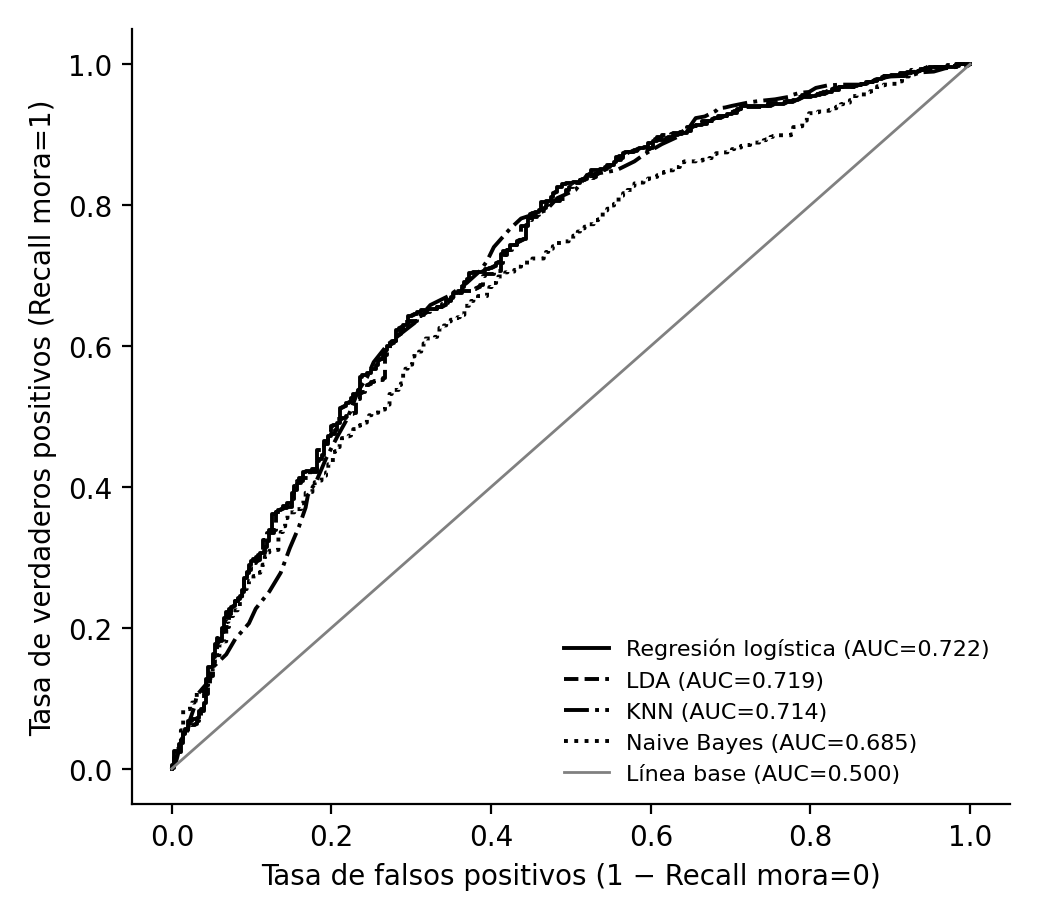
\includegraphics[width=0.72\textwidth]{fig_roc.png}
  \caption{Curvas ROC en el conjunto de prueba.}
  \label{fig:roc}
\end{figure}

\begin{figure}[H]
  \centering
  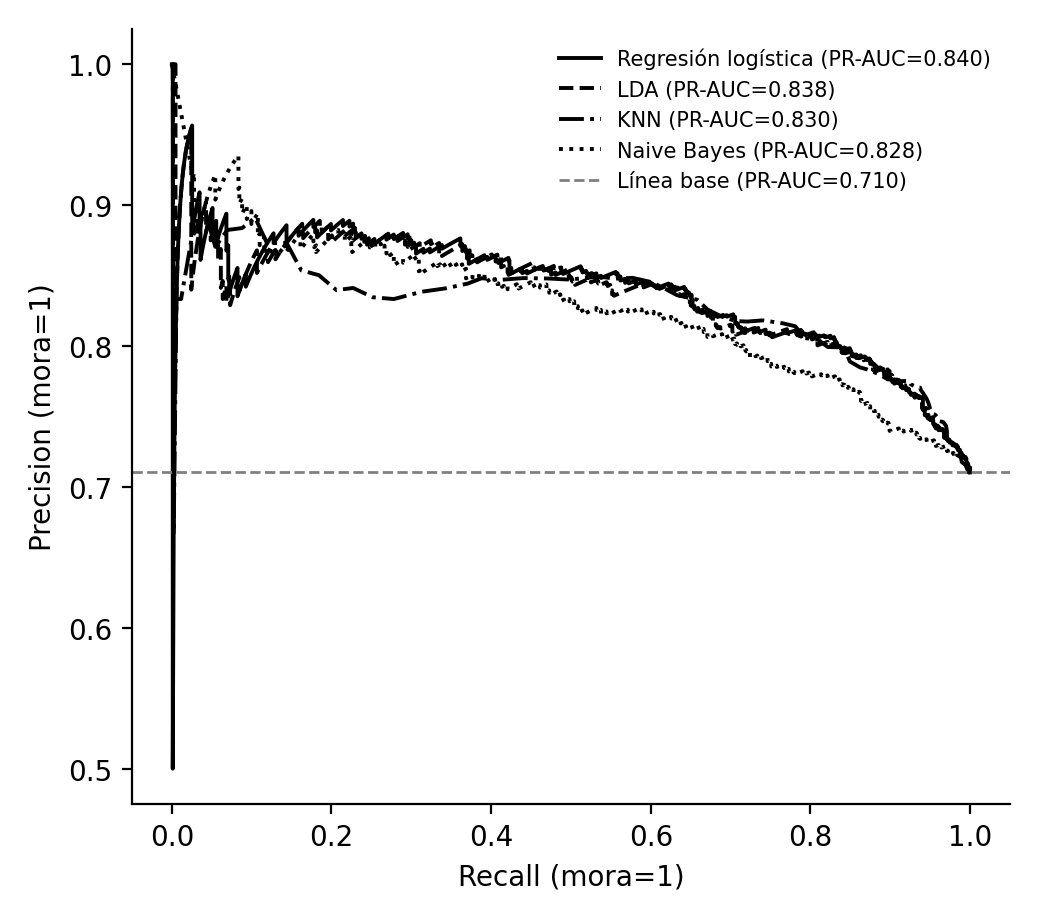
\includegraphics[width=0.72\textwidth]{fig_pr.png}
  \caption{Curvas precision--recall en prueba. La línea horizontal es la prevalencia de mora ($\approx$0,71).}
  \label{fig:pr}
\end{figure}

Los tres modelos principales suben el AUC de 0,5 a $\approx$0,72; Naive Bayes a 0,685. Con umbral 0,5 la logística detecta casi todos los morosos pero rechaza muchos buenos pagadores; con Youden OOF el equilibrio mejora en especificidad, a costa de más FN. Cuál conviene depende del costo de cada error para el banco, y esta base no lo dice.

\section{Sensibilidad a las variables sospechosas}

\begin{table}[H]
  \centering
  \caption{AUC en prueba por escenario.}
  \label{tab:sens}
  \small
  \begin{tabular}{@{}lccc@{}}
    \toprule
    Modelo & A completo & B principal & C sin score \\
    \midrule
    Regresión logística & 0,734 & 0,722 & 0,709 \\
    LDA & 0,730 & 0,719 & 0,707 \\
    KNN & 0,721 & 0,714 & 0,702 \\
    Naive Bayes & 0,692 & 0,685 & 0,677 \\
    \bottomrule
  \end{tabular}
\end{table}

Incluir \texttt{atraso} y \texttt{clasif\_sbs} sube el AUC unos 0,007--0,012, menos que la variación de la CV. Nos quedamos con el escenario B por ser más seguro.

\section{Interpretación preliminar y supuestos}

Usamos coeficientes de la logística principal (Figura~\ref{fig:coef}) solo como asociaciones en esta muestra, no como causas. Separamos supuestos del modelo (binaria, independencia de filas, linealidad con el \textbf{logit}, VIF bajo), decisiones de preprocesamiento y supuestos sobre calidad de datos (71\% de mora no es prevalencia real en Perú).

\begin{figure}[H]
  \centering
  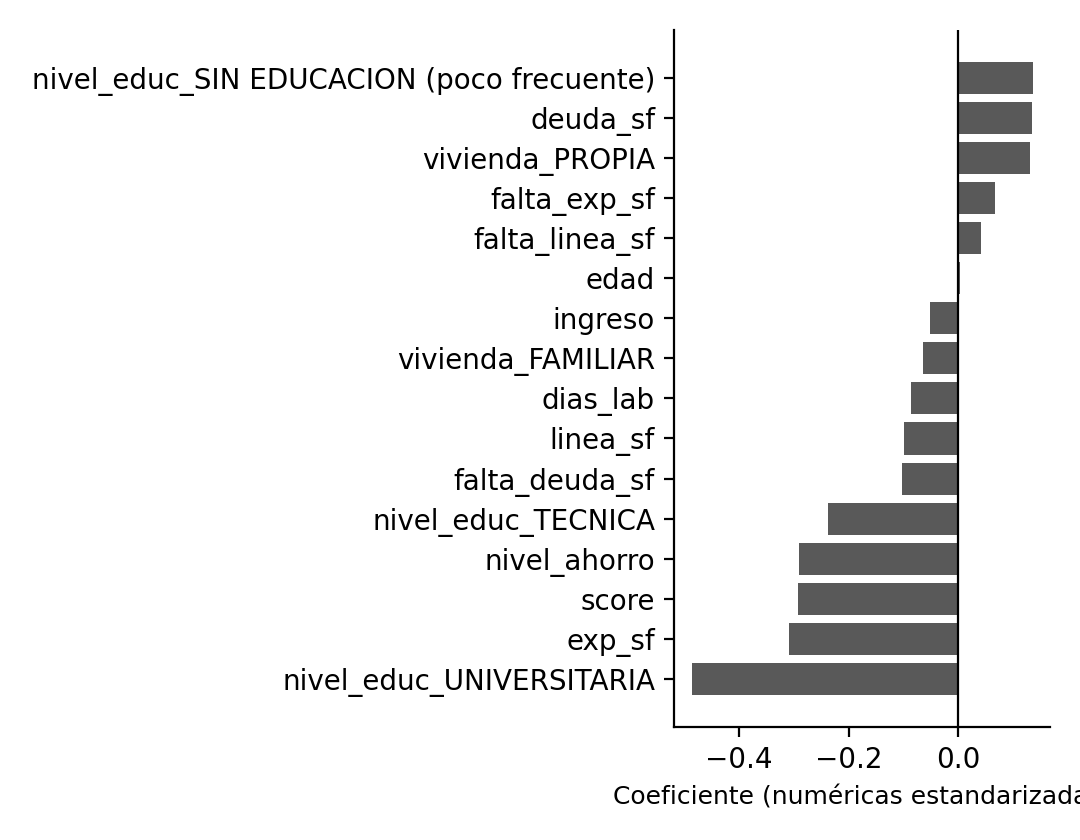
\includegraphics[width=0.78\textwidth]{fig_coeficientes.png}
  \caption{Coeficientes de la regresión logística (sin zonas).}
  \label{fig:coef}
\end{figure}

\section{Limitaciones, próximos pasos y chequeo de rúbrica}

\begin{itemize}
  \item Sin diccionario: definición de \texttt{mora} y momentos son supuestos.
  \item Probabilidades del modelo ordenan clientes; no son prevalencia poblacional.
  \item Sin fechas ni ID de cliente: no hay validación temporal.
  \item Para la entrega final: QDA y regularización (Ridge/Lasso), si el curso lo cubre; comparar costos de error para elegir umbral operativo.
\end{itemize}

\begin{table}[H]
  \centering
  \caption{Chequeo frente a la rúbrica de la segunda entrega.}
  \label{tab:rubrica}
  \small
  \begin{tabular}{@{}p{3.8cm}p{8.8cm}@{}}
    \toprule
    Criterio & Evidencia en informe y notebook \\
    \midrule
    Fuga y definición de \texttt{mora} & Secciones 2--3; escenarios A/B/C \\
    Pipeline reproducible & Sección 4; semilla 42; sin ajustar con prueba \\
    Balanceo & Tabla~\ref{tab:balanceo}; ROC-AUC y PR-AUC \\
    Validación y umbral & CV $k=5$; Youden solo con OOF en train; prueba una vez \\
    Análisis & Tablas~\ref{tab:test}--\ref{tab:sens}; figuras~\ref{fig:roc} y \ref{fig:pr} \\
    Sustentación & Este informe + notebook ejecutable \\
    \bottomrule
  \end{tabular}
\end{table}

\section*{Declaración de uso de inteligencia artificial}
Usamos Claude como apoyo para código, cálculos y borradores; el equipo revisó el planteamiento, las decisiones de diseño y la interpretación. Somos responsables del contenido final.

\begin{thebibliography}{9}
\bibitem{anthropic} Anthropic. (2026). Claude [Modelo de lenguaje]. \url{https://claude.ai}
\bibitem{attota} Attota, D. C., \& Yarmohammadtoosky, S. (2024). Optimizing Fintech Marketing (arXiv:2412.16333).
\bibitem{kaggle} Calderón Baldeón, L. H. (2021). BankDefaultAnalysis. Kaggle.
\bibitem{sbs} SBS Perú. Estadísticas de morosidad. \url{https://www.sbs.gob.pe}
\end{thebibliography}

\end{document}
